\documentclass{article}
\usepackage[utf8]{inputenc}
\usepackage{graphicx}
\graphicspath{{./img/}}
\author{Sebastian Ellefsen}
\title{%
		Datamaskiner og Digitalteknikk 2018 \\
		\large TDT4160}

\begin{document}
	\maketitle
	\section{Forelesing 1 - Introduksjon}
		\subsection{TL;DR}
			\begin{itemize}
				\item Prosessorhastighet vokser mye raskere enn minnehastigheten, lager et "gap", behov for å "lure" maskinen til å tro at den er raskere enn den er.
				\item Maskiner brytes ned til et abstrakt hierarki.
			\end{itemize}
	\section{%
		Forelesing 2 \\
		\small Mikroarkitektur}
		\subsection{Datamaskinsystemer}
			\begin{itemize}
				\item To typer maskiner
					\begin{itemize}
						\item Tradisjonelle datamaskiner
						\item Integrerte ("embedded") maskiner 
					\end{itemize}
			\end{itemize}
		\subsection{System og minnekart}
			\begin{itemize}
				\item Pekere til forskjellige minneområder
			\end{itemize}
			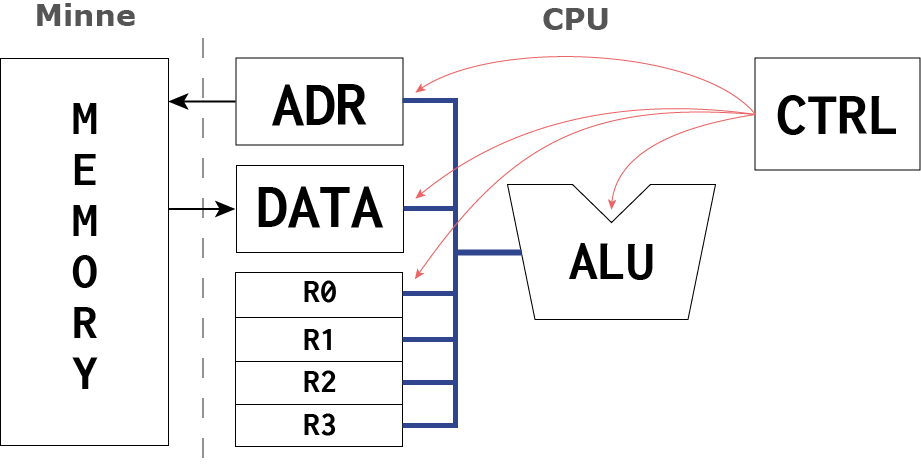
\includegraphics[width=\textwidth]{blokkdiagram.png} \\
			ADR holder pekere til minneadresser i DATA, data kan da skrives til minne (WR) eller leses fra minne (RD) 
		\subsection{CPU}
			\begin{itemize}
				\item "Hjernen" i en datamaskin
				\item Hoveddeler
					\begin{itemize}
						\item Control Unit
						\item Aritmetisk-logisk enhet (ALU)
						\item Register
							\begin{itemize}
								\item PC : Program counter \\
									\small Peker til den neste instruksjonen i Instruksjons Registeret
								\item MAR : Memory Address Register \\
									\small Lagrer adressen data enten vil hentes (fetch) fra eller skrives (write/send) til.
								\item MDR : Memory Data Register \\
									\small Lagrer data som flyttes til/fra primærminne
								\item Y-REG : 
								\item MUX : (multiplexer?)
								\item IR : Instruction Register (Instruksjons Register) \\
									\small Lagrer instruksjonene som skal utføres
								\item R0 ... R(n-1) : General Purpose Registers (GPRs) / Generelle register \\
									\small Registre som brukes av instruksjonene
								\item TEMP \\
									\small Brukes til forskjellige formål av forskjellige produsenter
								\item Konstant-register \\
									\small Lagrer en del read-only konstanter, f.eks 0, 1, $\pi$ etc.
							\end{itemize}
					\end{itemize}
				\item Register
					\begin{itemize}
						\item Programteller (PC) - Adresse til neste instruksjon
						\item Instruksjonsregister (IR)
						\item Generelle registre (General Purpose Registers (GPRs))
					\end{itemize}
			\end{itemize}
		\subsection{Hvordan utføres et program}
			\begin{itemize}
				\item Fetch-Execute cycle
				\item Programminne og Dataminne
			\end{itemize}
		\subsection{Lager}
			Hovedminne / Main Memory
			\begin{itemize}
				\item RAM (Random Access Memory)
				\item To vanlige typer RAM
					\begin{itemize}
						\item Statisk
							\begin{itemize}
								\item Rask
								\item Stor minecelle (Mange transistorer)
							\end{itemize}
						\item Dynamisk
							\begin{itemize}
								\item Ikke så rask
								\item Mindre minneareal
								\item Mer komplisert
								\item Må ha "opplading" (bruker kondensatorer som kan lades ut)
							\end{itemize}
					\end{itemize}
			\end{itemize}
			Lagerhierarki (hastighet$\downarrow$ / kapasitet $\uparrow$ 
			
			\begin{itemize}
				\item Register
				\item Cache
				\item Main Memory
				\item Magnetic DIsk
				\item Tape / Optical Disk
			\end{itemize}
		Nærmere CPU $\rightarrow$ Raskere / mindre
			\subsubsection{Cache}
				Mean Access Time: $x + (1 - h) \cdot m$
				Prøver gjette hvilke data man trenger
				\begin{itemize}
					\item c: cache access time
					\item m: main mamory acces time
					\item m: hit ratio
				\end{itemize}
			\subsection{Busser og arkitektur}
				Busser forbinder komponenter.
			\subsection{Ytelse}
				Må velge hvilken metrikk vi bruker for måling av ytelse, avhengig av behov.
			\subsection{Paral6lellitet}
				\begin{itemize}
					\item Essensielt for å øke ytelsen
					\item To typer parallellitet
						\begin{itemize}
							\item Instruksjonsnivåparallellitet (Instruction-Level Parallelism (ILP))
								\begin{itemize}
									\item Flere instruksjoner utføres samtidig
									\item Samlebånd (pipelining)
								\end{itemize}
							\item Prosessornivåparallellitet (Processor-Level Paralellism (PLP))
								\begin{itemize}
									\item Bruker flere prosessorer
								\end{itemize}
						\end{itemize}
				\end{itemize}
				Parallellitetstyper:
				\begin{itemize}
					\item  Single Instruction, Multiple Data (SIMD): Array Processor
					\item Multiple Instructions, Multiple Data (MIMD): Multiprocessor
				\end{itemize}
		\end{document}